\documentclass[aspectratio=169]{beamer}
\usetheme{Madrid}
\usecolortheme{dolphin}

\usepackage{booktabs}
\usepackage{xcolor}
\usepackage{listings}
\usepackage{graphicx}
\usepackage{tikz}
\usepackage{amsmath}

\definecolor{myblue}{RGB}{41,98,158}
\definecolor{mygreen}{RGB}{46,125,50}
\definecolor{myred}{RGB}{183,28,28}
\definecolor{codebg}{RGB}{13,17,23}
\definecolor{codefg}{RGB}{201,209,217}
\definecolor{mygray}{RGB}{100,100,100}

\setbeamercolor{frametitle}{bg=myblue,fg=white}
\setbeamercolor{structure}{fg=myblue}
\setbeamertemplate{navigation symbols}{}

\lstset{
  backgroundcolor=\color{codebg},
  basicstyle=\ttfamily\scriptsize\color{codefg},
  keywordstyle=\color{cyan},
  commentstyle=\color{gray!80},
  language=C, frame=none, tabsize=2,
  breaklines=true, showstringspaces=false
}

\title[LLM + Formal Verification]{When Does Prompting Help LLMs\\
Write Formal Verification Specifications?}
\author[SpecVerify Extension paper]{Weiqi}
\institute[]{Supervisors: Prof.\ Lucas Cordeiro \& Dr.\ Marie Farrell}
\date{\today}

\begin{document}

% ── 1. Title ──────────────────────────────────────────────────────────────────
\begin{frame}
  \titlepage
\end{frame}

% ── 2. Hook ───────────────────────────────────────────────────────────────────
\begin{frame}{The Problem: Passing $\neq$ Complete}

\begin{columns}[T]

\column{0.52\textwidth}

\begin{center}
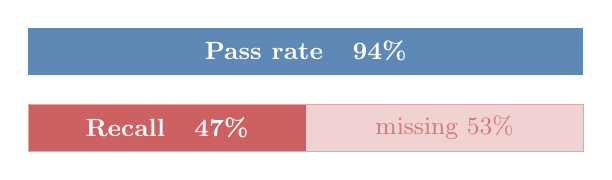
\begin{tikzpicture}[scale=0.75]
  \fill[myblue!75] (0,1.3) rectangle (9.4,2.1);
  \node[font=\small\bfseries, text=white] at (4.7,1.7) {Pass rate\quad 94\%};
  \fill[myred!70]  (0,0)   rectangle (4.7,0.8);
  \fill[myred!20]  (4.7,0) rectangle (9.4,0.8);
  \draw[myred!40, thin] (0,0) rectangle (9.4,0.8);
  \node[font=\small\bfseries, text=white] at (2.35,0.4) {Recall\quad 47\%};
  \node[font=\small, text=myred!60] at (7.05,0.4) {missing 53\%};
\end{tikzpicture}
\end{center}

\medskip
{\small\color{mygray} 238 expert CBMC harnesses · aws-c-common + s2n-tls}

\column{0.45\textwidth}

\begin{itemize}\small
  \item CBMC only checks what you specify
  \item LLM harness compiles and passes \checkmark
  \item But \textbf{53\% of GT properties missing}\\
        — the ones that catch subtle bugs
\end{itemize}

\bigskip
\textcolor{myred}{\textbf{Passing CBMC $\neq$ Complete Specification}}

\end{columns}

\end{frame}

% ── 3. Pipeline ───────────────────────────────────────────────────────────────
\begin{frame}{Experimental Pipeline}
\begin{center}
  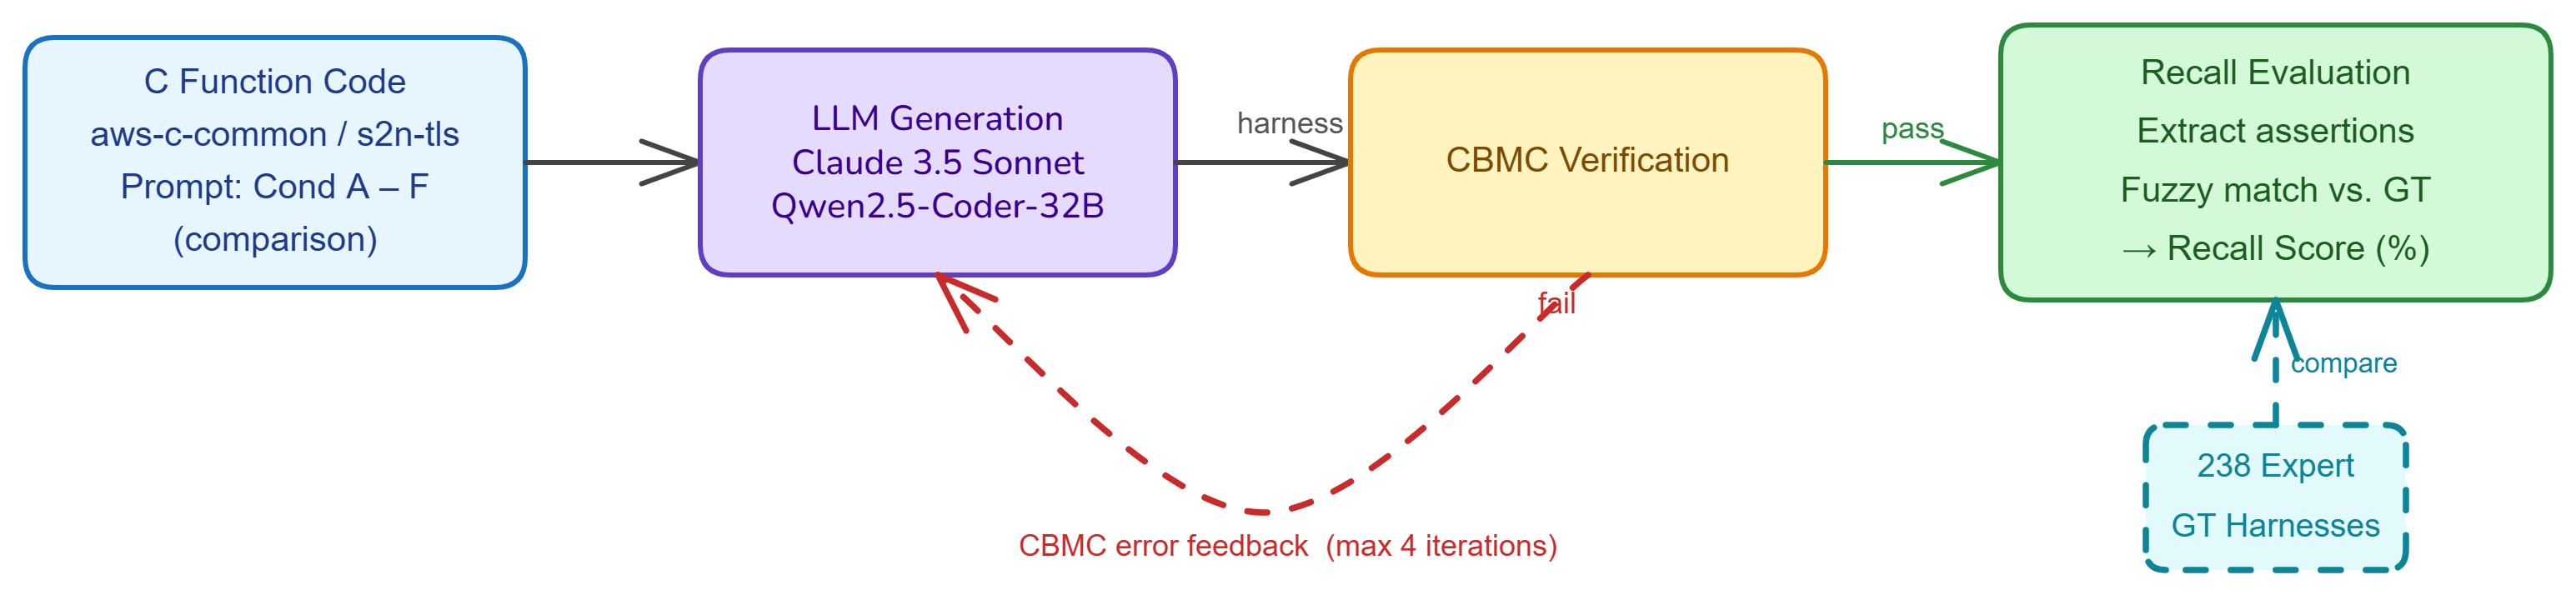
\includegraphics[width=0.92\textwidth]{figures/research_pipeline.png}
\end{center}
\end{frame}

% ── 4. Research Questions ─────────────────────────────────────────────────────
\begin{frame}{Research Questions}

\begin{columns}[T]

\column{0.50\textwidth}
\begin{block}{RQ1 — Baseline Completeness}
{\small How complete are LLM-generated verification harnesses,\\
and what types of properties are systematically missed?}
\end{block}

\smallskip
\begin{block}{RQ2 — Text Prompting}
{\small Does providing NL documentation or chain-of-thought\\
reasoning improve postcondition recall?}
\end{block}

\column{0.47\textwidth}
\begin{block}{RQ3 — Few-shot Example}
{\small Does a same-family GT harness example improve recall,\\
and what mechanisms drive the improvement?}
\end{block}

\smallskip
\begin{block}{RQ4 — Feedback Loop}
{\small Does iterative verifier error feedback improve recall?}
\end{block}

\smallskip
{\tiny\color{mygray}
Current study: CBMC (aws-c-common, s2n-tls) \quad·\quad
Extension: ESBMC}

\end{columns}

\end{frame}

% ── 5. Recall Metric ──────────────────────────────────────────────────────────
\begin{frame}{How We Measure Recall}

\begin{columns}[T]

\column{0.50\textwidth}
\textbf{Mechanism:}
\begin{enumerate}\small
  \item Extract all \texttt{assert(...)} from GT and LLM harnesses via regex
  \item Apply semantic normalization:
  \begin{itemize}\small
    \item Equality direction: \texttt{a==b} $\leftrightarrow$ \texttt{b==a}
    \item Pointer access: \texttt{list->len} $\leftrightarrow$ \texttt{list.len}
    \item Old-state naming: \texttt{old\_x} $\leftrightarrow$ \texttt{x\_old}
  \end{itemize}
  \item $\text{Recall} = |\text{matched}| \;/\; |\text{GT}|$
\end{enumerate}

\medskip
{\small\color{myblue}
\textbf{Conservative lower bound} — mismatches only\\
under-count recall, never over-count.}

\column{0.47\textwidth}
\textbf{Known limitations:}
\begin{itemize}\small
  \item \texttt{AWS\_OP\_SUCCESS} $\neq$ \texttt{0} (macro not expanded)
  \item \texttt{assert(a \&\& b)} $\neq$ two separate asserts
  \item[$\Rightarrow$] True recall $\geq$ measured recall
\end{itemize}

\medskip
\textbf{Planned validation:}
\begin{itemize}\small
  \item \textcolor{mygray}{Manual spot-check: $\sim$30 matched/unmatched pairs}
  \item \textcolor{mygray}{Taxonomy annotation: blind inter-rater + Cohen's $\kappa$}
\end{itemize}

\end{columns}

\end{frame}

% ── 5. Diagnosis ──────────────────────────────────────────────────────────────
\begin{frame}[fragile,shrink=18]{Why the Gap: CBMC Idioms}

\begin{columns}[T]
\column{0.48\textwidth}
{\color{myred}\textbf{LLM harness}} — passes, but incomplete:
\begin{lstlisting}
void aws_byte_buf_init_harness() {
  size_t capacity = nondet_size_t();
  __CPROVER_assume(capacity > 0);
  struct aws_byte_buf buf;
  aws_byte_buf_init(&buf, alloc, capacity);

  assert(buf.capacity == capacity);
  assert(buf.len == 0);
}
\end{lstlisting}

\column{0.48\textwidth}
{\color{mygreen}\textbf{Ground truth}} — 4 missing assertions:
\begin{lstlisting}
// Validity predicate:
assert(aws_byte_buf_is_valid(&buf));

// Frame condition:
assert(buf.allocator == alloc);

// Struct invariant:
assert(buf.len <= buf.capacity);

// Pointer coherence:
assert(buf.buffer != NULL
       || buf.capacity == 0);
\end{lstlisting}
\end{columns}

\medskip
{\small\renewcommand{\arraystretch}{1.1}
\begin{tabular}{lrl}
\toprule
\textbf{Category} & \textbf{\%} & \textbf{Why missed} \\
\midrule
VALIDITY\_PRED & 20\% & predicate name unknown \\
LEN\_INVARIANT & 19\% & struct contract unknown \\
FRAME\_COND    & 17\% & LLM focuses on changes \\
\midrule
\textbf{Top 3} & \textbf{56\%} &
  \textcolor{myred}{\textbf{Tool-specific idiom gap — not misunderstanding the function}} \\
\bottomrule
\end{tabular}}


\end{frame}

% ── 5. Text fails, Example works ──────────────────────────────────────────────
\begin{frame}[shrink=8]{Text Cannot Teach Idioms — Examples Can}

\begin{columns}[T]

\column{0.50\textwidth}
\begin{block}{\textbf{Text Prompting: No Effect}}
{\small\renewcommand{\arraystretch}{1.2}
\resizebox{\columnwidth}{!}{%
\begin{tabular}{lcc}
\toprule
\textbf{Condition} & \textbf{Claude} & \textbf{Qwen} \\
\midrule
A: baseline    & 46\% & 39\% \\
B: + NL docs   & 47\% & 40\% \\
C: + CoT       & 47\% & 35\% \\
D: + NL + CoT  & 45\% & 38\% \\
\midrule
$p$ vs A & \multicolumn{2}{c}{$> 0.28$} \\
\bottomrule
\end{tabular}}}

\medskip
{\small\color{myred} Ceiling $\sim$47\% — tool-specific idioms, not fixable by text}\\[4pt]
{\tiny\color{mygray} $p$: Wilcoxon signed-rank test vs.\ baseline (Cond.\ A)}
\end{block}

\column{0.47\textwidth}
\begin{block}{\textbf{One Same-Family Example: +9pp}}
{\small\renewcommand{\arraystretch}{1.2}
\resizebox{\columnwidth}{!}{%
\begin{tabular}{lcc}
\toprule
\textbf{Setting} & \textbf{A} & \textbf{E (+ example)} \\
\midrule
Claude / aws & 46\% & \textbf{56\%} ($p{=}0.002$) \\
Qwen / aws   & 39\% & \textbf{47\%} ($p{=}0.037$) \\
Qwen / s2n   & 42\% & \textbf{51\%} ($p{=}0.003$) \\
\bottomrule
\end{tabular}}}

\medskip
{\small\color{mygreen} Free $\cdot$ No retraining $\cdot$ Replicates}
\end{block}

\end{columns}

\end{frame}

% ── 6. Replication ────────────────────────────────────────────────────────────
\begin{frame}{Replicated Across Models and Libraries}

\begin{columns}[T]

\column{0.52\textwidth}
\begin{center}
  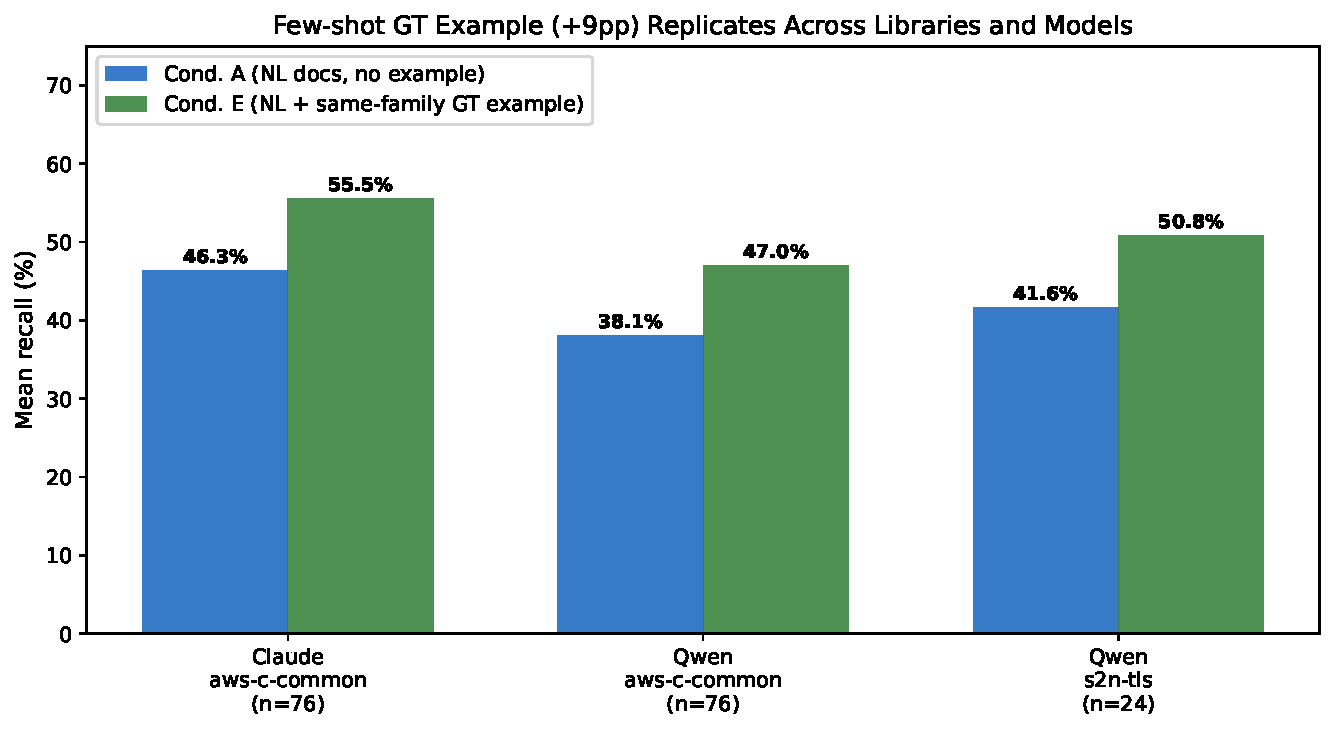
\includegraphics[width=\textwidth]{figures/replication.pdf}
\end{center}

\column{0.45\textwidth}

{\small\renewcommand{\arraystretch}{1.3}
\begin{tabular}{lcc}
\toprule
\textbf{Setting} & $\boldsymbol{\Delta}$ & $\boldsymbol{p}$ \\
\midrule
Claude / aws & $+$9.2pp & 0.002 \\
Qwen / aws   & $+$8.9pp & 0.037 \\
Qwen / s2n   & $+$9.5pp & 0.003 \\
\bottomrule
\end{tabular}}

\medskip
{\small\color{myblue}
\begin{itemize}
  \item 2 models, 2 libraries
  \item Effect size $r = 0.6$ (large)
  \item Not a fluke
\end{itemize}}

\end{columns}

\end{frame}

% ── 7. Take-away + Open Questions ─────────────────────────────────────────────
\begin{frame}{Take-away \& Open Questions}

\begin{columns}[T]

\column{0.52\textwidth}

\begin{block}{\centering Recommendation}
\begin{center}
{\normalsize Always include one same-family\\[3pt]
GT harness in the prompt.}\\[6pt]
{\small Free $\cdot$ Replicable $\cdot$ $+$9pp recall}
\end{center}
\end{block}

\medskip
{\small
\textbf{Two mechanisms (ablation F):}\\[4pt]
\quad \textcolor{myblue}{(1) Generic idioms:} any example $\rightarrow$ $+$5.8pp\\
\quad \textcolor{mygreen}{(2) Predicate names:} same family $\rightarrow$ $+$15pp
}

\column{0.45\textwidth}

\textbf{Open Questions:}
\begin{itemize}\small
  \item How many examples? (1 vs.\ 2--3)
  \item Generate example when no GT exists?
  \item Feedback paradox: recall flat as pass rises
  \item Generalise to ESBMC + Simulink?
\end{itemize}


\end{columns}

\end{frame}

\end{document}
